% 中文 TikZ 重排：坐标及曲线提取自原 PDF，未重新模拟数据。
\begin{figure}[htbp]
\centering
\definecolor{chfourfig1c0}{rgb}{1.0,1.0,1.0}
\definecolor{chfourfig1c1}{rgb}{0.13669,0.12195,0.12529}
\definecolor{chfourfig1c2}{rgb}{0.84295,0.84816,0.85371}
\definecolor{chfourfig1c3}{rgb}{0.77444,0.78143,0.78912}
\definecolor{chfourfig1c4}{rgb}{0.18155,0.18994,0.57328}
\definecolor{chfourfig1c5}{rgb}{0.93042,0.1109,0.14145}
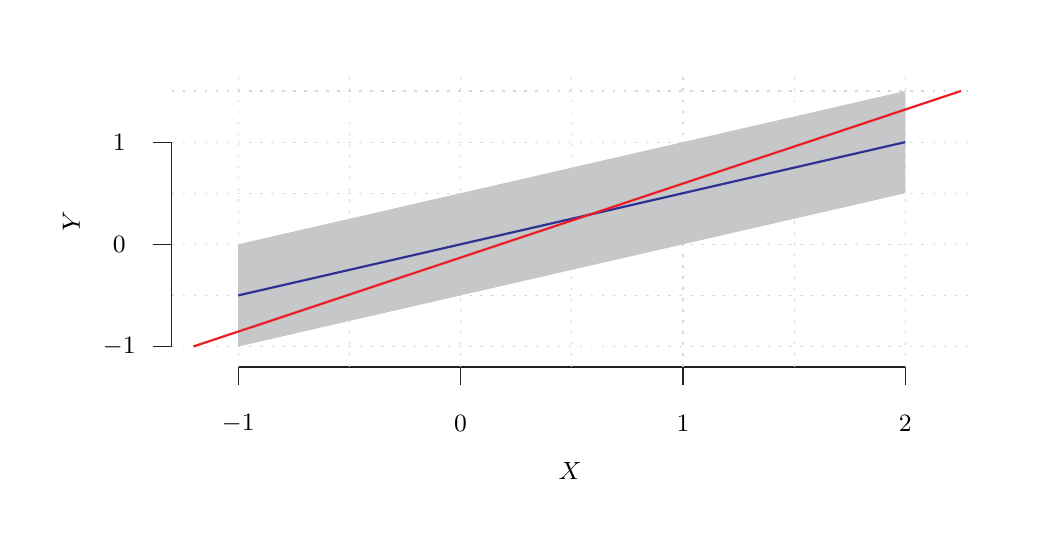
\begin{tikzpicture}[x=0.043cm,y=-0.043cm]
\useasboundingbox (0,0) rectangle (290,144);
\path[fill=chfourfig1c0,fill opacity=1.0,draw=none] (42.4942,100.2089) --(42.4942,12.6660) --(278.9107,12.6660) --(278.9107,100.2089) --(42.4942,100.2089);
\path[fill=none,draw=chfourfig1c1,line width=0.3985pt,draw opacity=1.0] (42.4942,94.1714) --(42.4942,33.7971);
\path[fill=none,draw=chfourfig1c1,line width=0.3985pt,draw opacity=1.0] (42.4942,94.1714) --(37.1143,94.1714);
\path[fill=none,draw=chfourfig1c1,line width=0.3985pt,draw opacity=1.0] (42.4942,63.9843) --(37.1143,63.9843);
\path[fill=none,draw=chfourfig1c1,line width=0.3985pt,draw opacity=1.0] (42.4942,33.7971) --(37.1143,33.7971);
\path[fill=none,draw=chfourfig1c1,line width=0.3985pt,draw opacity=1.0] (62.1906,100.2089) --(259.2044,100.2089);
\path[fill=none,draw=chfourfig1c1,line width=0.3985pt,draw opacity=1.0] (62.1906,100.2089) --(62.1906,105.5888);
\path[fill=none,draw=chfourfig1c1,line width=0.3985pt,draw opacity=1.0] (127.8652,100.2089) --(127.8652,105.5888);
\path[fill=none,draw=chfourfig1c1,line width=0.3985pt,draw opacity=1.0] (193.5398,100.2089) --(193.5398,105.5888);
\path[fill=none,draw=chfourfig1c1,line width=0.3985pt,draw opacity=1.0] (259.2044,100.2089) --(259.2044,105.5888);
\path[fill=none,draw=chfourfig1c2,line width=0.3985pt,draw opacity=1.0,dash pattern=on .99628pt off 2.98883pt] (62.1906,100.2089) --(62.1906,12.6660);
\path[fill=none,draw=chfourfig1c2,line width=0.3985pt,draw opacity=1.0,dash pattern=on .99628pt off 2.98883pt] (95.0279,100.2089) --(95.0279,12.6660);
\path[fill=none,draw=chfourfig1c2,line width=0.3985pt,draw opacity=1.0,dash pattern=on .99628pt off 2.98883pt] (127.8652,100.2089) --(127.8652,12.6660);
\path[fill=none,draw=chfourfig1c2,line width=0.3985pt,draw opacity=1.0,dash pattern=on .99628pt off 2.98883pt] (160.7025,100.2089) --(160.7025,12.6660);
\path[fill=none,draw=chfourfig1c2,line width=0.3985pt,draw opacity=1.0,dash pattern=on .99628pt off 2.98883pt] (193.5398,100.2089) --(193.5398,12.6660);
\path[fill=none,draw=chfourfig1c2,line width=0.3985pt,draw opacity=1.0,dash pattern=on .99628pt off 2.98883pt] (226.3671,100.2089) --(226.3671,12.6660);
\path[fill=none,draw=chfourfig1c2,line width=0.3985pt,draw opacity=1.0,dash pattern=on .99628pt off 2.98883pt] (259.2044,100.2089) --(259.2044,12.6660);
\path[fill=none,draw=chfourfig1c2,line width=0.3985pt,draw opacity=1.0,dash pattern=on .99628pt off 2.98883pt] (42.4942,94.1714) --(278.9107,94.1714);
\path[fill=none,draw=chfourfig1c2,line width=0.3985pt,draw opacity=1.0,dash pattern=on .99628pt off 2.98883pt] (42.4942,79.0778) --(278.9107,79.0778);
\path[fill=none,draw=chfourfig1c2,line width=0.3985pt,draw opacity=1.0,dash pattern=on .99628pt off 2.98883pt] (42.4942,63.9843) --(278.9107,63.9843);
\path[fill=none,draw=chfourfig1c2,line width=0.3985pt,draw opacity=1.0,dash pattern=on .99628pt off 2.98883pt] (42.4942,48.8907) --(278.9107,48.8907);
\path[fill=none,draw=chfourfig1c2,line width=0.3985pt,draw opacity=1.0,dash pattern=on .99628pt off 2.98883pt] (42.4942,33.7971) --(278.9107,33.7971);
\path[fill=none,draw=chfourfig1c2,line width=0.3985pt,draw opacity=1.0,dash pattern=on .99628pt off 2.98883pt] (42.4942,18.7035) --(278.9107,18.7035);
\path[fill=chfourfig1c3,fill opacity=1.0,draw=none] (62.1906,94.1714) --(259.2044,48.8907) --(259.2044,18.7035) --(62.1906,63.9843) --(62.1906,94.1714);
\path[fill=none,draw=chfourfig1c4,line width=0.7970pt,draw opacity=1.0] (62.1906,79.0778) --(259.2044,33.7971);
\path[fill=none,draw=chfourfig1c5,line width=0.7970pt,draw opacity=1.0] (48.9402,94.1714) --(275.6629,18.7035);
\node[font=\small,inner sep=0pt,rotate=0] (ch04f1t0) at (27.0451,94.1727) {$-1$};
\node[font=\small,inner sep=0pt,rotate=0] (ch04f1t1) at (27.0451,63.9855) {$0$};
\node[font=\small,inner sep=0pt,rotate=0] (ch04f1t2) at (27.0451,33.7985) {$1$};
\node[font=\small,inner sep=0pt,rotate=0] (ch04f1t3) at (62.1903,117.0401) {$-1$};
\node[font=\small,inner sep=0pt,rotate=0] (ch04f1t4) at (127.8635,117.0401) {$0$};
\node[font=\small,inner sep=0pt,rotate=0] (ch04f1t5) at (193.5376,117.0401) {$1$};
\node[font=\small,inner sep=0pt,rotate=0] (ch04f1t6) at (259.2016,117.0401) {$2$};
\node[font=\small,inner sep=0pt,rotate=0] (ch04f1t7) at (160.2394,130.8567) {$X$};
\node[font=\small,inner sep=0pt,rotate=90] (ch04f1t8) at (12.8868,57.3129) {$Y$};
\end{tikzpicture}
\caption{一个可识别例子中 $X,Y$ 的联合密度。蓝线表示正向模型 $Y:=0.5X+N_Y$ 所对应的函数，其中 $X,N_Y$ 均服从均匀分布；灰色区域表示 $(X,Y)$ 密度的支撑集。定理4.2表明，由于 $(X,N_Y)$ 的分布为非高斯分布，不可能存在有效的反向模型。由 $(b,c)$ 刻画的红线是使 $\EE[(X-bY-c)^2]$ 最小的最小二乘拟合。它并不构成有效的反向模型 $X=bY+c+N_X$，因为所产生的噪声 $N_X$ 不会与 $Y$ 独立：$N_X$ 支撑集的大小随 $Y$ 的取值而改变。}
\label{fig:ch04-1}
\end{figure}
